%\documentclass[pra,superscriptaddress,twocolumn]{revtex4-1}[11pt] 
\documentclass[article]{revtex4-1}[11pt] 
\pdfoutput=1
\usepackage{amsmath,amssymb,graphicx} 
\usepackage{hyperref}
\usepackage{color}
%\usepackage[normalem]{ulem}
%\usepackage{epsf,verbatim}
%\usepackage{comment}



\begin{document} 


%\title{Increasing particle discrimination in dark matter searches using liquid xenon emission detectors}
\title{Detection of primary scintillation photons dominates particle discrimination in liquid xenon}
\author{P. Sorensen, others?}
%\thanks{pfs@llnl.gov}
%\affiliation{LUX Collaboration internal note}
%\affiliation{Lawrence Berkeley National Laboratory, 1 Cyclotron Rd., Berkeley, CA 94720, USA} 
 
\begin{abstract}
This is a study of $\beta/\gamma$ event versus neutral particle event discrimination in liquid xenon emission detectors. A simple model is developed and used to show that a key factor in obtaining better discrimination is the efficiency for collecting scintillation photons. The model predicts the possibility that discrimination could be perhaps three orders of magnitude better than the present state-of-the-art $\sim(1-10^{-3})$. 
\\
\\
\end{abstract}
\date{\today}

\maketitle

 %\setcounter{equation}{0} \setcounter{footnote}{0}

%%%%%%%%%%%%%%%%%%%%%%%%%%%%%%%%%%%%%%%%%%%%%%%%%%%
\section{{Introduction}}\label{sec:intro}
Liquid xenon emission detectors are a variant of the time projection chamber in which ionized electrons are drifted to the liquid-gas interface, extracted and amplified via proportional scintillation. This technique affords single electron sensitivity. The collection of 175~nm scintillation photons is more challenging, but is aided by the high reflectivity Teflon and photomultipliers whose quantum efficiency now exceeds $\sim30\%$. The details of the operation of this class of detectors have been explained in detail elsewhere (see e.g. \cite{}), and herein are briefly reviewed. 

Excellent rare-event search capability may be obtained with these detectors because (among other features) they can be made highly radio-pure and they can localize event vertices in $(x,y,z)$. For dark matter searches, it is also critical that they have a detection threshold of about 1 keV and can discriminate background events from expected signal. This is obtained from the ratio of detected electrons to photons, $n_e/n_{\gamma}$. The scintillation signal arrives first in time and so is typically referred to as $S1 = n_{\gamma} g_1$, where $g_1$ is the total efficiency for photon detection. The electron signal is delayed by an amount proportional to the electron drift time and is typically referred to as $S2=n_e g_2 \eta$, where $g_2$ is the effective gain factor for a single electron and $\eta$ is its probability to be emitted from the liquid into the gas. 

The discrimination of $\beta/\gamma$ events from neutral particle events is obtained from the fact that the ratio $d=n_e/n_{\gamma}$ depends on the specific energy loss $dE/dx$. It is commonly written as $d=\mbox{log}_{10}(S2/S1)$.  Events due to natural radioactivity are unavoidable in a counting experiment, so the power of this discriminant is of keen interest to dark matter searches. The experimental sensitivity to interactions due to hypothetical dark matter particles from our galactic halo has been increasing faster than Moore's Law \cite{}. The field contains many different technologies operating in a variety of underground laboratories around the world. At present, the LUX experiment at Sanford Underground Research Facility in South Dakota is the most sensitive search. The planned LZ experiment (to be installed in the same facility) may find it's sensitivity limited by electron scattering events due to solar proton-proton chain neutrinos.

This is a remarkable state of affairs, in that a measurement of proton-proton chain solar neutrinos in the 1-100~keV region would be a great achievement. And yet, it is somewhat troubling in terms of the aspiration to directly detect evidence of the particle nature of dark matter. The cross section of this hypothetical particle with ordinary matter remains unknown. Many models suggest a value at or below $10^{-48}$~cm$^2$, which would result in its scattering rate (and eventual detection) competing with solar neutrinos.

This is a study of $\beta/\gamma$ event versus neutral particle  (neutron, coherent neutrino, hypothetical dark matter) event discrimination in liquid xenon emission detectors. A simple model is developed and used to show that a key factor in obtaining better discrimination is the efficiency for collecting scintillation photons. The model predicts the possibility that discrimination could be perhaps three orders of magnitude better than the present state-of-the-art $\sim(1-10^{-3})$. This would be a boon to future dark matter searches, and will require new R\&D in photon sensing instrumentation.




\section{A simple model of liquid xenon emission detector response}\label{sec:model}
A model of the signal response of liquid xenon requires three basic ingredients: (a) the total number of quanta generated for a given energy deposit, (b) the partitioning of those quanta into ionized electrons and scintillation photons, and (c) the degree of fluctuation. %For item (a) we follow Shutt et al \cite{}, and for item (b) we follow Dahl \cite{}. However, it is necessary to make a slight modification to (and simplification of) his treatment in order to simply and effectively model the fluctuations. This modification distinguishes the present work from e.g. the NEST model \cite{}, which also followed Dahl.

\subsection{Basic components} \label{sec:model:basic}

The total number of quanta is related to the energy \cite{Shutt:2007zz} via
\begin{equation} \label{eq1}
E = w_q (n_e + n_{\gamma}) / f_n,
\end{equation}
where $w_q = 13.8\pm0.2$~eV \cite{Dahl:2009nta} is the average energy required to create a quanta, and $f_n$ is an energy-dependent quenching factor. This factor is $f_n \equiv1$ for $\beta/\gamma$ events, which are generally referred to as ``electron recoils.'' For neutral particle events, the dominant interaction is with the atomic nucleus. The energy loss process is that of a recoiling atom, but these events are often referred to as ``nuclear recoils'' (hence the subscript $n$). Their electromagnetic response is quenched, typically by about $1/5$. The Lindhard model of quenching gives a very reasonable approximation of this physical process \cite{Sorensen:2011bd}.

The slowing-down process involves a series of scattering events, distributed along a track. The result is a collection of ionized ($N_i$) and excited ($N_{ex}$) atoms. The applied electric field across the detector permits some fraction of the ionized electrons to be drifted away from their creation site, and measured. Excited atoms ($N_{ex}$) rapidly form dimers, which de-excite with the emission of a scintillation photon. This process is described in detail in \cite{Doke:1982}. Electron-ion pairs that recombine result in an excited atom, thus leading to an additional scintillation photon.

The initial creation of $N_i$ ionized atoms and $N_{ex}$ excited atoms is governed by the cross sections for ionization relative to atomic excitation, and should be different for electron recoils and nuclear recoils. In this work we specialize to the energy regime $E\lesssim10$~keV. The value of $N_{ex}/N_i$ is treated as a free parameter, constant for each type of recoil. Nuclear recoil data are well-fit by $N_{ex}/N_i=1.1$, which is consistent with the results obtained in \cite{}. For electron recoil data we take the calculated value \cite{} $N_{ex}/N_i=0.06$. 


It has been shown \cite{needref0} that the anti-correlation between $n_e$ and $n_{\gamma}$ has a slope of -1, which implies the equality
\begin{equation}\label{eq2}
n_e + n_{\gamma} = N_i + N_{ex}.
\end{equation}

Combining Eq. \ref{eq1} and Eq. \ref{eq2}, the  number of ionized atoms may be written as
\begin{equation} \label{eq3}
N_i = \frac{E f_n}{w_q(1+N_{ex}/N_i)},
\end{equation}

Dahl first showed \cite{Dahl:2009nta} that the amount of recombination was well-described by a modified version of the Thomas-Imel box model \cite{Thomas:1987zz}, which predicts a recombination probability for $N_i$ given by
\begin{equation}\label{eq4}
p = \frac{1}{\xi} \mbox{log}(1+\xi) \frac{N_i}{n_e+n_{\gamma}}, ~~~ \xi = \frac{\alpha N_i}{4a^2v}
\end{equation}
in which $\alpha$ is the recombination coefficient, the box which contains $N_i$ ions has sides of length $a$ and the electron velocity is $v$.

Here, a different modification of the box model is pursued. The box size and the recombination coefficient $\alpha$ are assumed to have a weak energy and field dependence. In practice, the combination $\alpha/a^2v$ is treated as a single free parameter. Its behavior is shown in Fig. \ref{yields}. 
\begin{figure}[h]
\begin{center}
\vskip -0.0cm
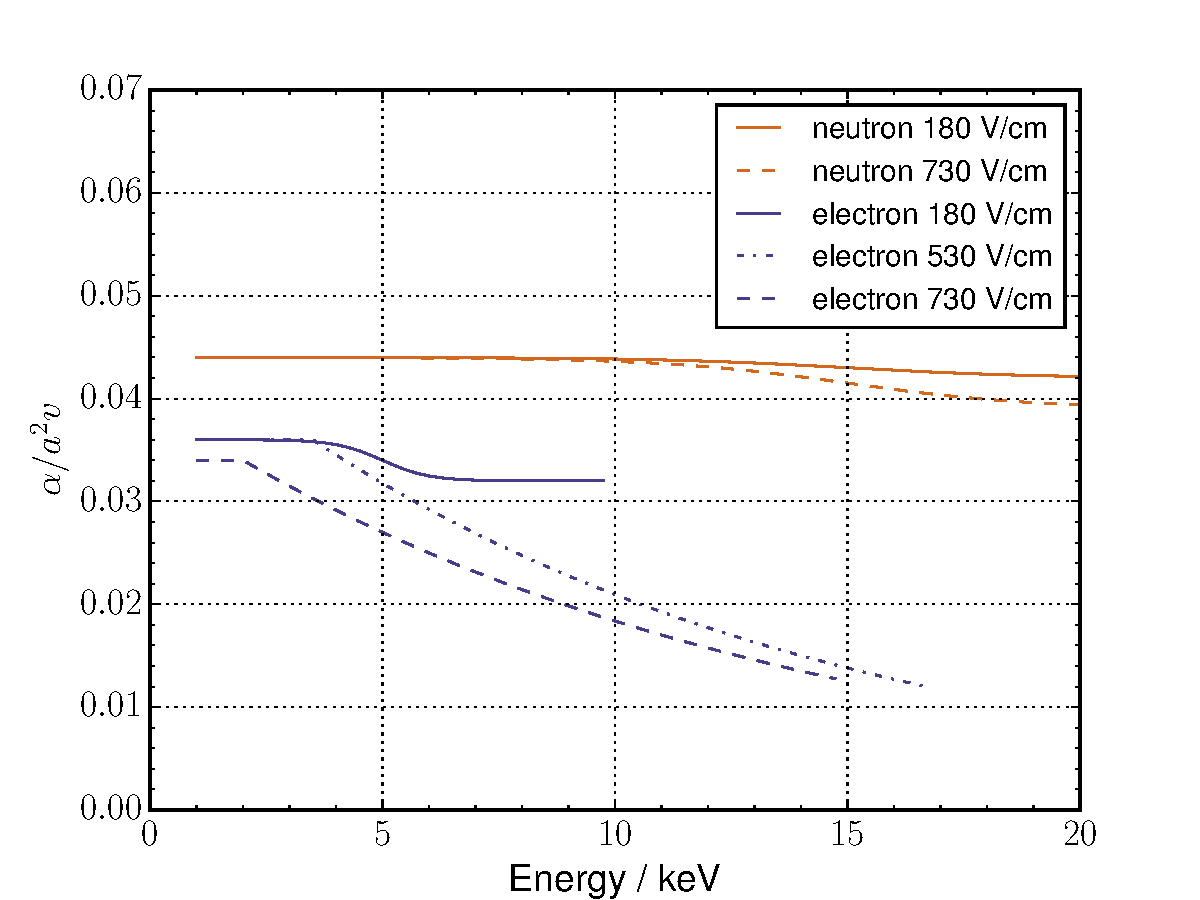
\includegraphics[width=0.48\textwidth]{figs/yields.pdf}
\vskip -0.1cm
\caption{}
\vskip -0.5cm
\label{yields}
\end{center}
\end{figure} 

A statistical simulation of a detector's response needs only model instrumental fluctuations (Sec. \ref{sec:model:meas}) and recombination fluctuations. Recombination fluctuations are given by the binomial probability for an ionized electron to recombine
\begin{equation}\label{eq5}
n_e = \binom{N_i}{p},
\end{equation}
For nuclear recoils, this description is sufficient. But for electron recoils, the observed fluctuations are greater than those described by Eq. \ref{eq5}. It must be that the variety of electron recoil tracks leads to additional fluctuation, whereas nuclear recoil tracks are sufficiently short and dense that no additional fluctuation is evident. This is both reasonable and consistent with our implementation of the box model, which ``neglects the coulomb forces entirely.'' 

Rather than start from a detailed electron recoil track Monte Carlo, we parameterize our ignorance by supposing that due to variations in track structure, the value of $p$ obtained by Eq. \ref{eq4} is actually the central value of a normal distribution with standard deviation $\sigma_p$. We use experimental data to determine $\sigma_p=0.07$, for tracks with energies $E>3$~keV. Below this energy, tracks are assumed to be too short to produce any significant fluctuation in recombination.

%These recombination fluctuations, together with the instrumental measurement fluctuations, fully reproduce the experimental width of the nuclear recoil response. 

%This simply states that the track recombination fluctuations are encompassed by $f_{e,1}$. It is a simple matter to ascertain the value of $f_{e,1}(E)$ by comparing with experimental data. The recombination fractions are shown in Fig. \ref{}.



\subsection{Instrumental measurement fluctuations} \label{sec:model:meas}
A series of additional binomial fluctuations are an inherent part of the measurement process. These are listed below. An $^*$ indicates that the process is not modeled in this work. After the initial recombination fluctuation,
\begin{itemize}
\item A fraction $g_1$ of photons create photo-electrons in the photomultipliers.
\item A small fraction of electrons are absorbed by impurities. $^*$
\item A fraction $\eta$ of electrons are extracted across the liquid-gas boundary.
\item Electrons drift through the gas, which creates several hundred scintillation photons. These photons impinge on the photomultipliers, and a fraction are converted to photoelectrons. A double photoelectron emission probability of 20\% is assumed based on \cite{Faham:2015kqa,Akerib:2015rjg}.
\item Detector response is a function of the physical position of the event. Results are reported with the response corrected to a single point in the detector. $^*$
\item Photomultipliers have an approximately 20\% probability to create two photoelectrons for each incident photon.
\end{itemize}

\section{Model versus data}
The model was tuned to reproduce the LUX ($E_d=180$~V/cm) and the XENON10 ($E_d=730$~V/cm) data sets. Data from XENON100 and ZEPLIN3 are discussed in the appendix. Two cautionary statements are in order. First, in the model there is some degeneracy between $N_{ex}/N_i$ and $\alpha/a^2v$, and therefore the absolute value of these parameters is not uniquely defined. Second, the experimental data from which Fig. \ref{yields} is derived may have their own systematic differences, for example in the software cuts that were applied. This points to the future importance of performing this sort of study on data from the same instrument.

\begin{figure}[h]
\begin{center}
\vskip -0.0cm
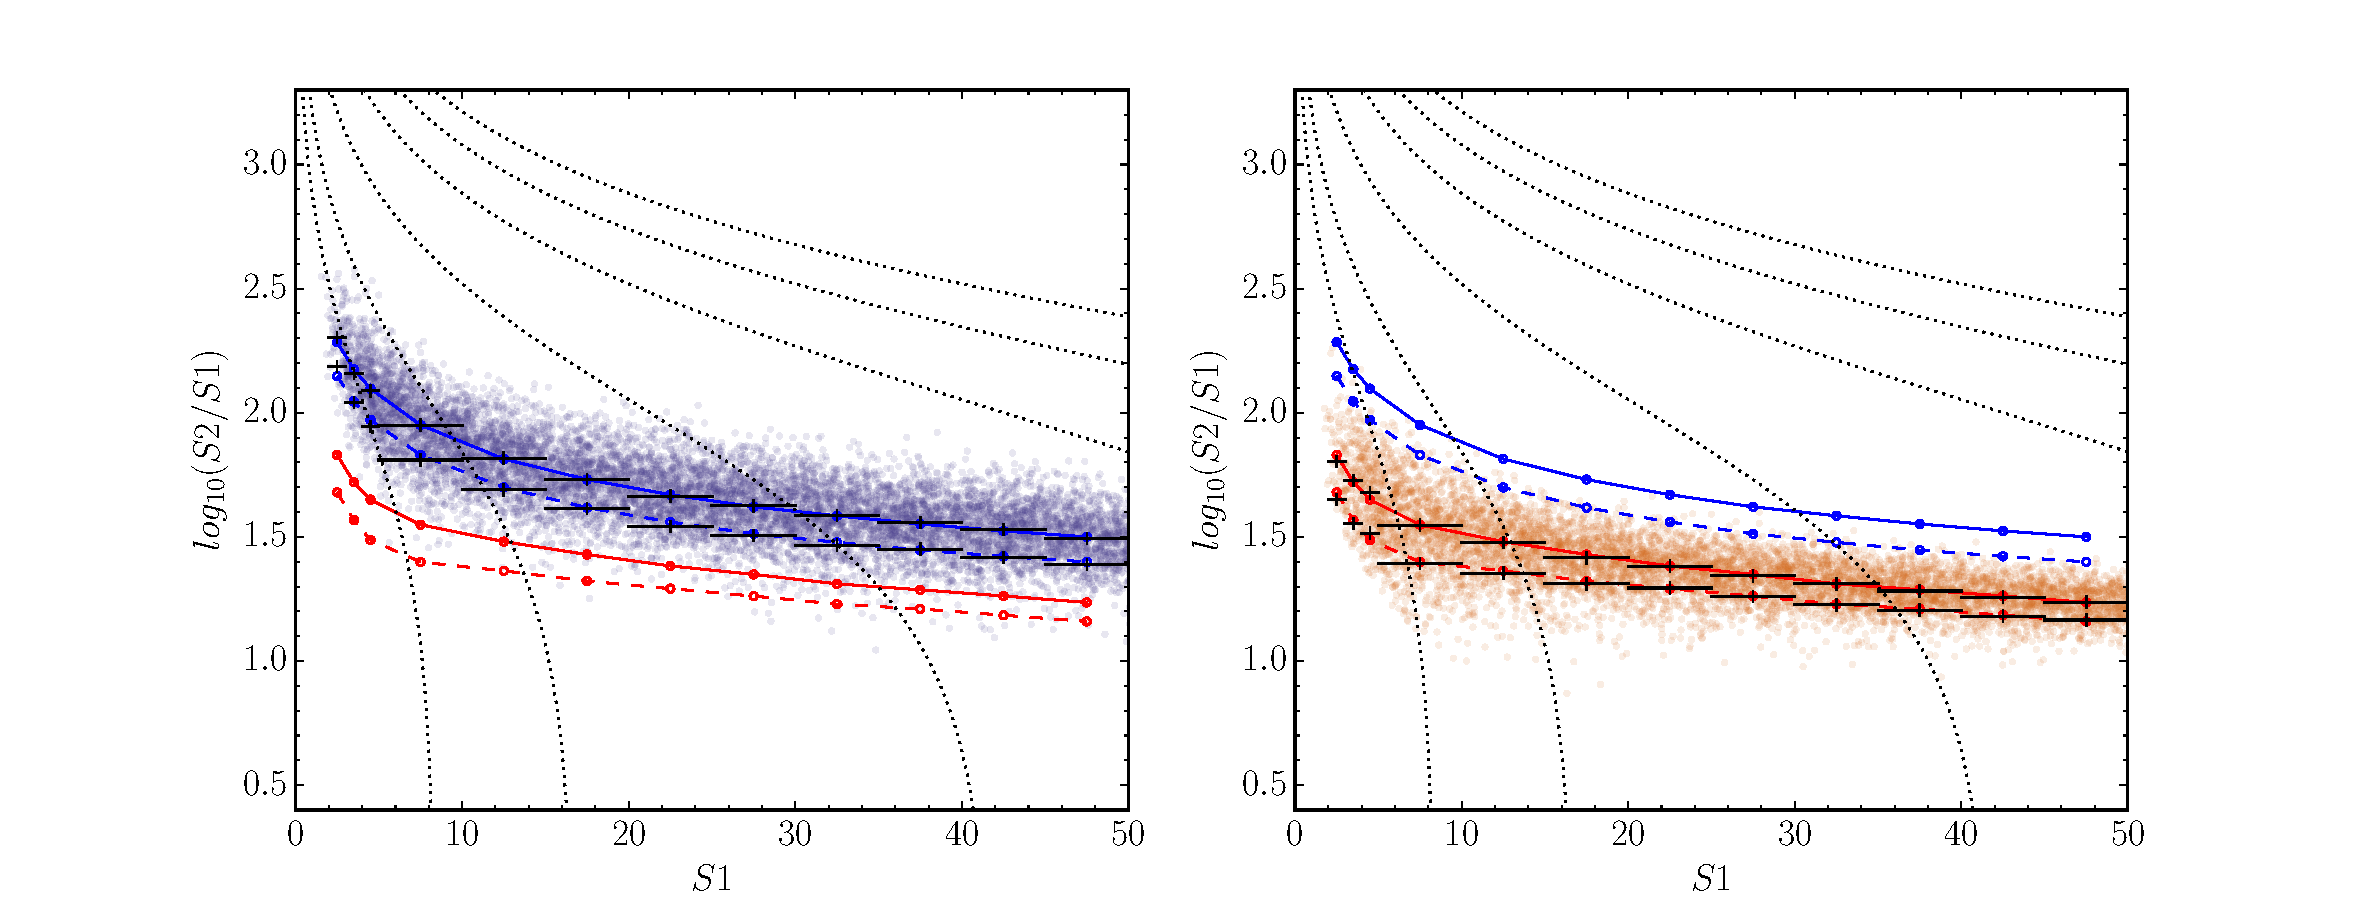
\includegraphics[width=0.95\textwidth]{figs/bands_LUX.pdf}
\vskip -0.1cm
\caption{Simulated events from the model for electron recoils (blue points, top band) and nuclear recoil (orange points, bottom band) at $E_d=180$~V/cm for a LUX-like detector. The black steps indicate $\mu$ and $-\sigma$ from a Gaussian fit. Blue and red curves indicate the same values obtained by the LUX Collaboration \cite{}.  }
\vskip -0.5cm
\label{bands_LUX}
\end{center}
\end{figure} 

\begin{figure}[h]
\begin{center}
\vskip -0.0cm
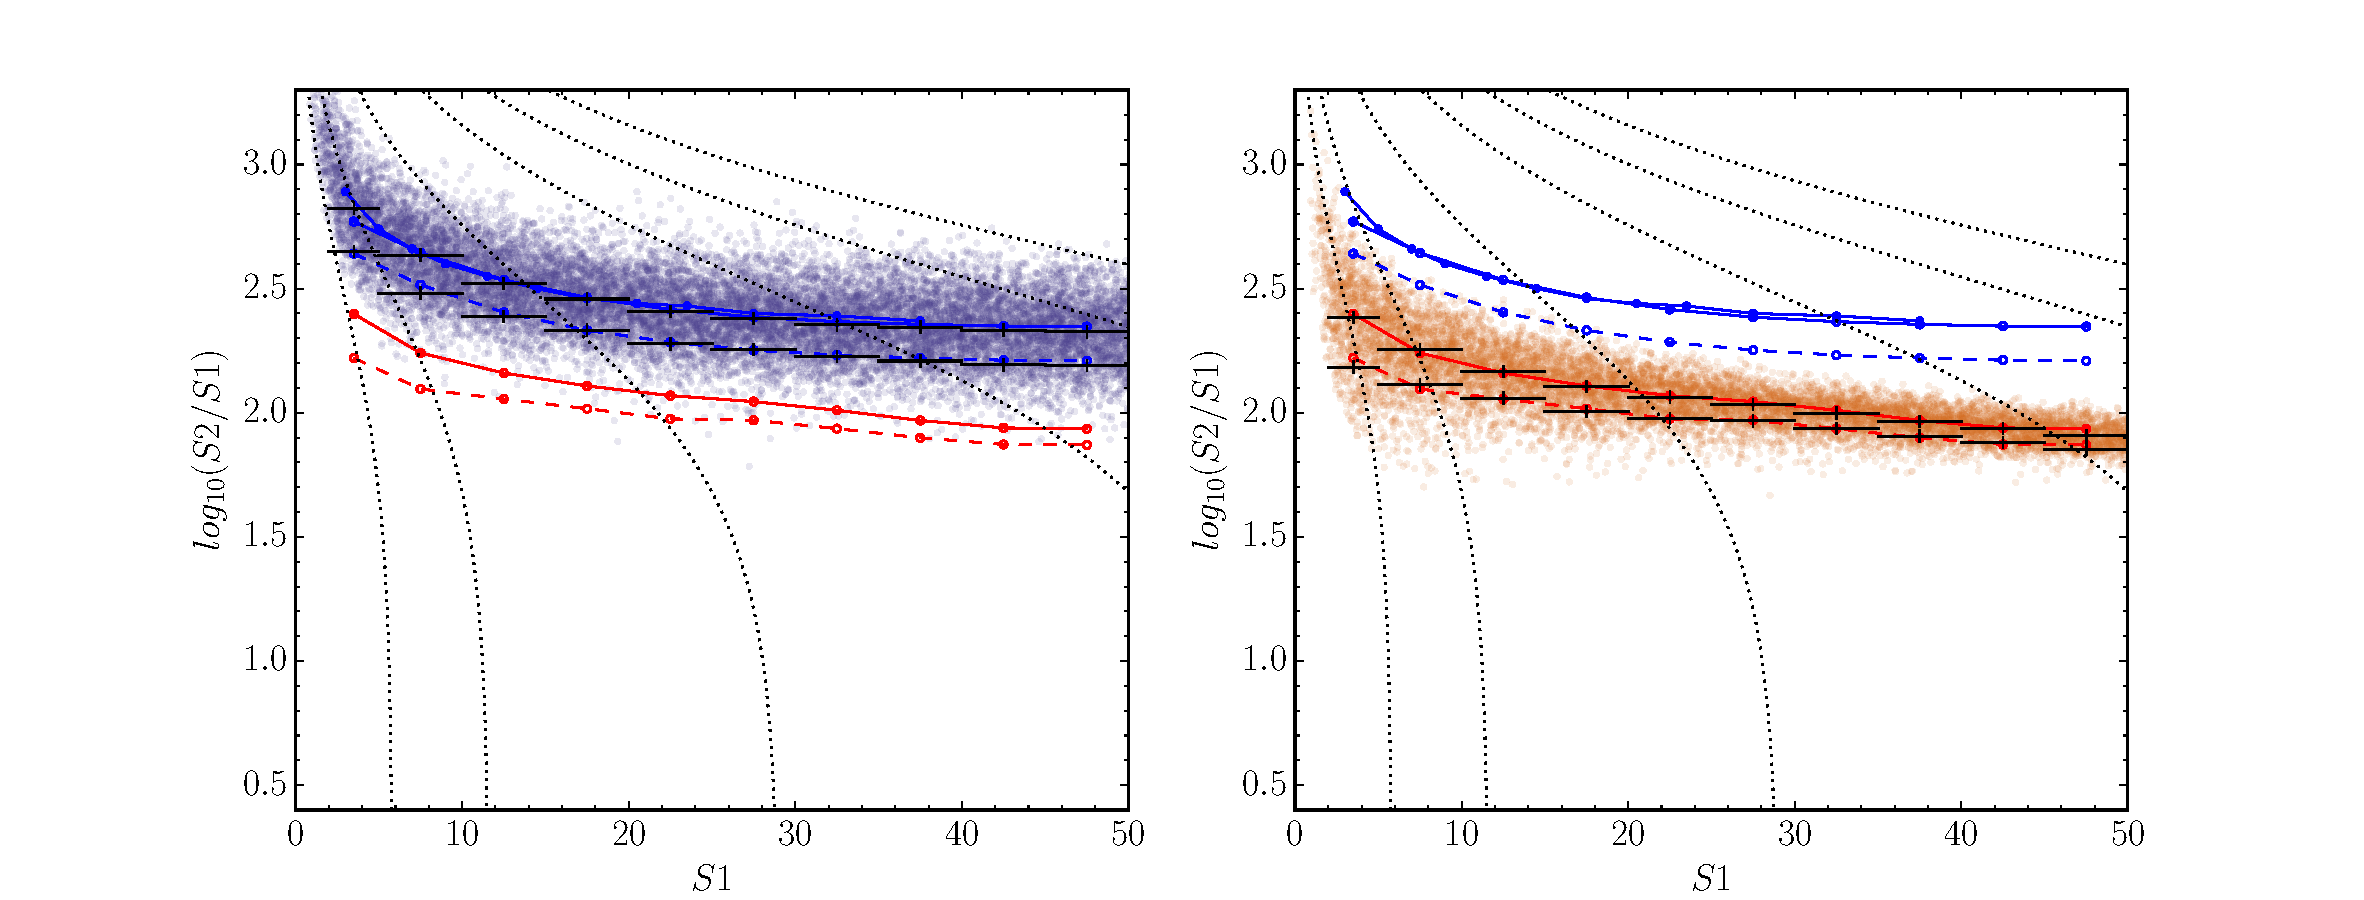
\includegraphics[width=0.95\textwidth]{figs/bands_XENON10.pdf}
\vskip -0.1cm
\caption{Simulated events from the model for electron recoils (blue points, top band) and nuclear recoil (orange points, bottom band) at $E_d=730$~V/cm for a XENON10-like detector. The black steps indicate $\mu$ and $-\sigma$ from a Gaussian fit. Blue and red curves indicate the same values obtained by the XENON10 Collaboration \cite{}. A second $\mu$ curve was obtained from \cite{} and is shown to indicate the range of systematic shift that software cuts may have on data.  }
\vskip -0.5cm
\label{bands_XENON10}
\end{center}
\end{figure} 

\section{The discrimination story}
$\times2$ in light collection is better than $\times3$ in field.

\begin{figure}[h]
\begin{center}
\vskip -0.0cm
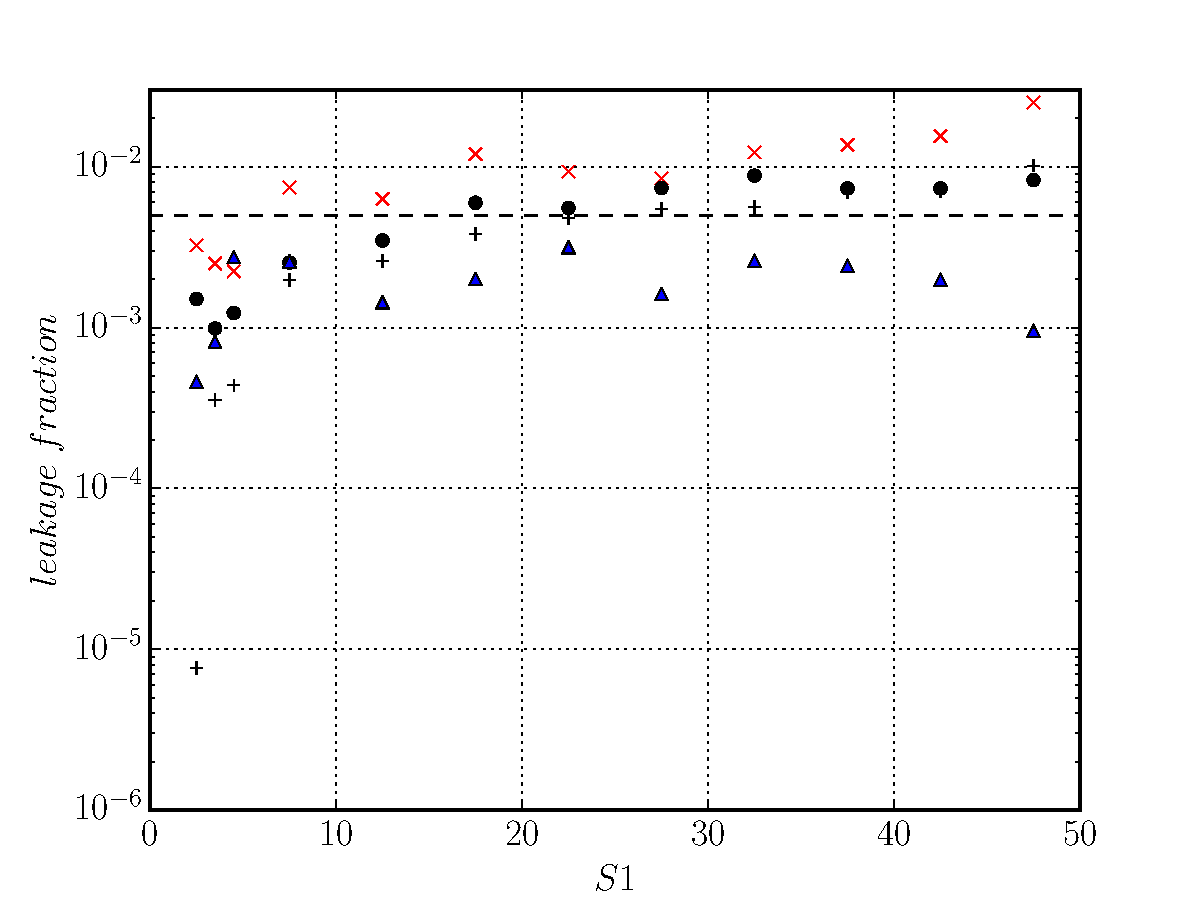
\includegraphics[width=0.95\textwidth]{figs/disc4.pdf}
\vskip -0.1cm
\caption{Discrimination projections for a LUX-like detector (Fig. \ref{bands_LUX}) as-built and operated (black circles); with $g_1=0.08$ instead of $g_1=0.117$ (red x); with $\eta=0.95$ instead of $\eta=0.50$ (grey +); and with $E_d=730$~V/cm instead of $E_d=180$~V/cm (blue triangles).  }
\vskip -0.5cm
\label{bands_XENON10}
\end{center}
\end{figure} 

\begin{figure}[h]
\begin{center}
\vskip -0.0cm
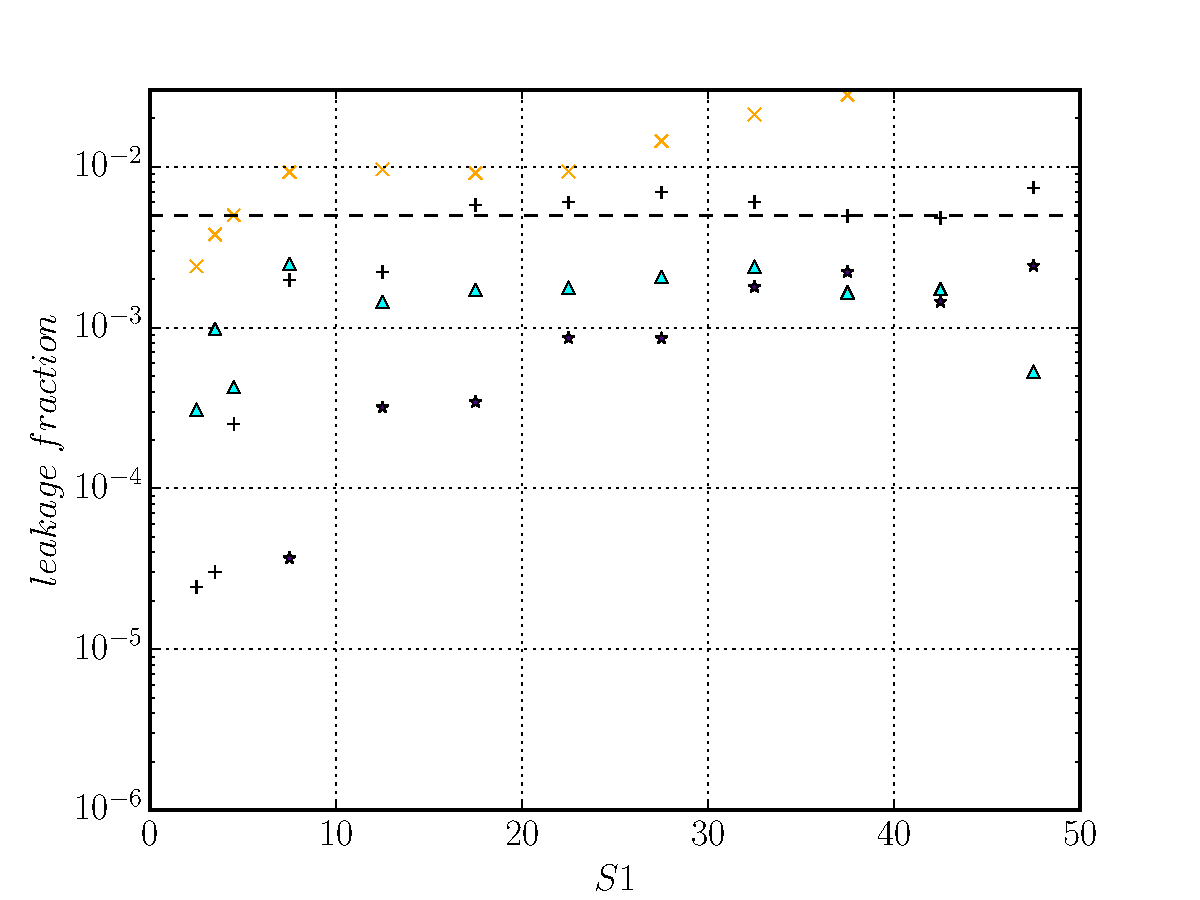
\includegraphics[width=0.95\textwidth]{figs/disc5.pdf}
\vskip -0.1cm
\caption{Discrimination projections for a LUX-like detector (Fig. \ref{bands_LUX}), but (in all cases) with $\eta=0.95$ instead of $\eta=0.50$. With $g_1=0.057$ instead of $g_1=0.117$ (orange x); with $g_1=0.117$ (grey +); with  $g_1=0.117$ and $E_d=730$~V/cm (cyan triangles); and with $g_1=0.234$ and $E_d=180$~V/cm (indigo stars).  }
\vskip -0.5cm
\label{bands_XENON10}
\end{center}
\end{figure} 




% \begin{table}[h]
%\centering
%\caption{Summary of the model prediction and data for gas phase xenon ($E_b=12.1$~eV), for incident electrons with $E_0=5.9$ keV.}
%\begin{tabular}{rlllcc}
%\\
%\toprule
%	  & $\epsilon$ (eV) & $F$ 	\\
%\hline
%model~   	& 21.3	  & 0.123	\\
%data~		& $21.7\pm0.5$ $^a$ & $0.15\pm0.02$ $^b$ \\
%\hline
%
%\hline
%\botrule
%\multicolumn{3}{l}{$^a$ Ref. \cite{Borges:1996}, $^b$ Ref. \cite{Nygren:2007zzc} }\\
%\end{tabular}
%\label{table1}
%\end{table}


%\clearpage{\pagestyle{empty}\cleardoublepage}

%\section{Appendix}


%%%%%%%%%%%%%%%%%%%%%%%%%%%%%%%%%%%%%%%%%%%%%%%%%%%


%%%%%%%%%%%%%%%%%%%%%%%%%%%%%%%%%%%%%%%%%%%%%%%%%%%


%\vskip 0.4 cm
%\begin{center} 
%{\bf Acknowledgements}
%\end{center}

\begin{thebibliography}{99}

\bibitem{Shutt:2007zz} 
  T.~Shutt, A.~Bolozdynya, P.~Brusov, C.~E.~Dahl and J.~Kwong, %``Performance and fundamental processes at low energy in a two-phase liquid xenon dark matter detector,''
  Nucl.\ Phys.\ Proc.\ Suppl.\  {\bf 173}, 160 (2007).
  doi:10.1016/j.nuclphysbps.2007.08.140
  %%CITATION = doi:10.1016/j.nuclphysbps.2007.08.140;%%

\bibitem{Dahl:2009nta} 
  C.~E.~Dahl, 
  Ph.D. Thesis, Princeton, NJ (2009) %``The physics of background discrimination in liquid xenon, and first results from Xenon10 in the hunt for WIMP dark matter,''
  AAT-3364532.
  %%CITATION = AAT-3364532;%%

\bibitem{Sorensen:2011bd} 
  P.~Sorensen and C.~E.~Dahl,
  %``Nuclear recoil energy scale in liquid xenon with application to the direct detection of dark matter,''
  Phys.\ Rev.\ D {\bf 83}, 063501 (2011)
  doi:10.1103/PhysRevD.83.063501
  [arXiv:1101.6080 [astro-ph.IM]].
  %%CITATION = doi:10.1103/PhysRevD.83.063501;%%

\bibitem{Thomas:1987zz} 
  J.~Thomas and D.~A.~Imel,
  %``Recombination of electron-ion pairs in liquid argon and liquid xenon,''
  Phys.\ Rev.\ A {\bf 36}, 614 (1987).
  doi:10.1103/PhysRevA.36.614
  %%CITATION = doi:10.1103/PhysRevA.36.614;%%

\bibitem{needref0}

\bibitem{Doke:1982}

\bibitem{Faham:2015kqa} 
  C.~H.~Faham, V.~M.~Gehman, A.~Currie, A.~Dobi, P.~Sorensen and R.~J.~Gaitskell,
  %``Measurements of wavelength-dependent double photoelectron emission from single photons in VUV-sensitive photomultiplier tubes,''
  JINST {\bf 10}, no. 09, P09010 (2015)
  doi:10.1088/1748-0221/10/09/P09010, 10.1088/1748-0221/2015/9/P09010
  [arXiv:1506.08748 [physics.ins-det]].
  %%CITATION = doi:10.1088/1748-0221/10/09/P09010, 10.1088/1748-0221/2015/9/P09010;%%
  
\bibitem{Akerib:2015rjg} 
  D.~S.~Akerib {\it et al.} [LUX Collaboration],
  %``Improved WIMP scattering limits from the LUX experiment,''
  arXiv:1512.03506 [astro-ph.CO].
  %%CITATION = ARXIV:1512.03506;%%
  
\end{thebibliography}


\end{document}













